This paper documents the authors' term project for SYSC5804: exploring channel reconstruction for m-MIMO systems. The study was based on NR communication systems simulated using MATLAB's 5G Toolbox. State-of-the-art channel reconstruction techniques were recreated in MATLAB and Python; methods include LASSO regression based approach \cite{Liu2016} and a YOLO image processing technique \cite{Li2020}. Additionally, the authors experimented with new methods, such as applying Deep Neural Network directly to the received pilots to predict the path gains, angles, and delays. This is an active research area for 5G systems that is both computationally and analytically complex. Some challenges arose that were not overcome within the time constraints of the course; however, there were many interesting results generated and the directions explored showed potential. The authors plan to continue this work in the future and hope to pursue a publication in the space. The remainder of this section will highlight the novel contributions from this work and the next steps for this research. Any feedback or suggestions for future work would be greatly appreciated! 

\subsection{Contributions}
Although this work was mostly focused on recreating stat-of-the-art channel reconstruction techniques there were several interesting contributions. Firstly, all the code for the channel simulator and the channel reconstruction algorithms implemented is freely available with documentation on GitHub \cite{git}. Prior work in this space has always kept the source code proprietary. Our project could act as the building blocks for future research in this space. The channel image generation algorithm is available, along with sample data sets that include the ground truth data for the paths. Additionally, several of these data sets have included YOLO bounding box labels validated manually, as well as pre-trained YOLO weights. Additionally, the antenna based analysis of LASSO performance was novel. Prior researchers had not shown how LASSO performance was affected by antennas count. Studying the ideal antenna configurations for LASSO regression analysis could be valuable future research.  

\subsection{Future Work} 

The authors believe there is potential to use DNNs to improve the state-of-the-art image based path recognition from the received pilots. First, it would be interesting to explore how DNN image processing methods compared to classical methods such as LASSO in low SNR scenarios. A full analysis and performance comparison between the two techniques would generate worthwhile results. Additionally, \cite{Li2020} uses YOLO to detect points in the image, it would be interesting to apply DNNs to the problem directly. This was already investigated as part of the project, without results. This is largely due to how resource intensive State-of-the-art deep learning solutions are. With more time and some better resources we believe models can be made to go directly from received pilots in either time-antenna or delay-phase space to the path components. Furthermore, there was a thought to explore using DNNs to solve the implementation problem in the YOLO method. Instead of mathematically going from the pixel coordinates to the path delays and angles, a DNN could predict these values. It may not be as effiecent, although it would be interesting to see if the algorithm could solve the math problems that we could not.

Classical image processing techniques may improve path detection. There are likely faster algorithms for high SNR scenarios, since the paths are more obvious. It would be interesting to study using classical computer vision techniques and a hybrid technique that combines classical object detection with deep learning \cite{mahony2019}. For instance, performing a convolution on the image with a sharpening matrix will make the faint paths far more apparent, simplifying their extraction from the image. Another interesting approach would be applying a threshold, changing all pixels under it to black and over it to white. This threshold can be scaled up or down until there is a desired number of paths in the image. This is shown in figure \ref{fig:thld}, where the paths are far clearer in the image after applying the threshold. 

\begin{figure}[H]
    \subfigure[]{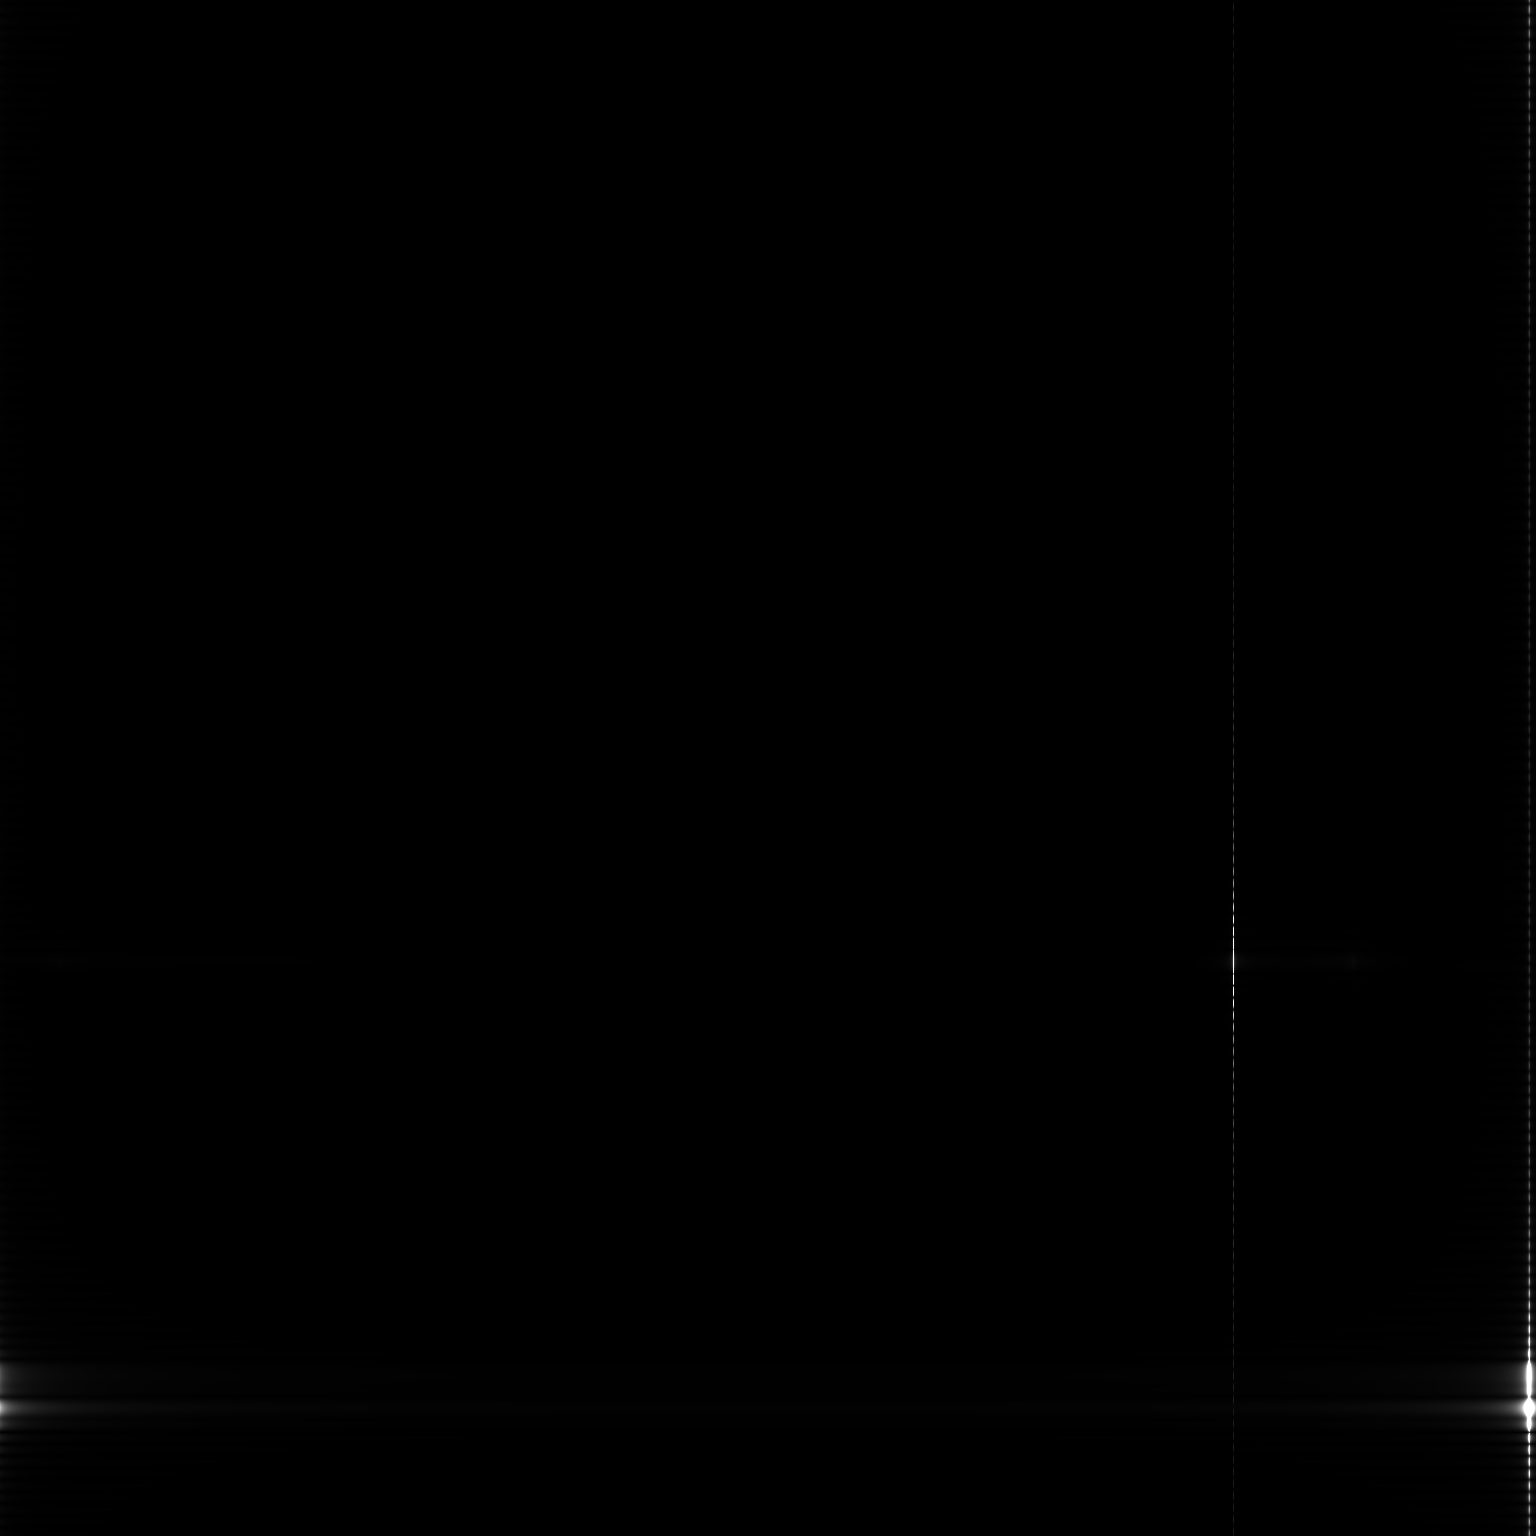
\includegraphics[width=0.49\textwidth]{91.png}} 
    \subfigure[]{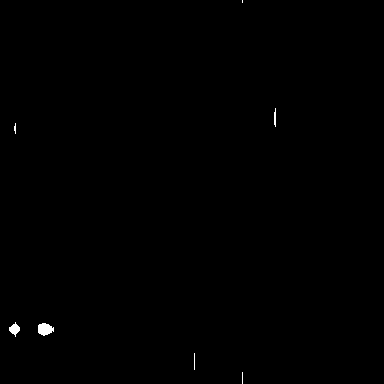
\includegraphics[width=0.49\textwidth]{figures/91_threshold.png}}
    \caption{Threshold Example (a) Original Image (b) After Applying Threshold}
    \label{fig:thld}
\end{figure}
\noindent

Finally, we are interested in exploring how these algorithms will expand to other antenna array configurations. All the novel m-MIMO channel reconstruction techniques use uniform linear arrays of antennas to simplify the model. This is good for a proof of concept; however, it is not a practical assumption, as any m-MIMO deployed will not have all its antennas in a single line. Supporting more complex antennas arrays will require extrapolating the math into higher dimension, since a single angle will not fully represent the path. A deeper understanding of antenna configurations and the channel reconstruction math is required before we can explore this avenue.